\documentclass[conference]{IEEEtran}

\usepackage{cite}
\usepackage{amsmath}
\usepackage{url}
\usepackage{hyperref}
\hypersetup{hidelinks}
\usepackage{booktabs}
\usepackage{multirow}
\usepackage{graphicx}
\usepackage{listings}
\usepackage[table]{xcolor}
\usepackage{tikz}
\usepackage{flushend}
\usetikzlibrary{arrows.meta,positioning,shapes.geometric}

\lstdefinestyle{prompt}{
  basicstyle=\ttfamily\fontsize{7}{7.8}\selectfont,
  breaklines=true,
  columns=fullflexible,
  frame=single,
  framerule=0.3pt,
  xleftmargin=0.4em,
  xrightmargin=0.4em,
  aboveskip=0.35em,
  belowskip=0.35em,
  showstringspaces=false
}

\title{Reproducing and Extending TISER:\\
Context--Memory Conflict and Tennis-Domain Adaptation for Temporal Reasoning}

\author{
\IEEEauthorblockN{
Gabriele Adorni s349308,
Alessandro Casadei s349386, \\
Taha Atabay Cetin s349501
}
\IEEEauthorblockA{
Politecnico di Torino\\
Deep Natural Language Processing
}
}

\begin{document}

\maketitle

\begin{abstract}
Temporal reasoning requires a model to organise events before answering questions about order, duration, and overlap. We implement and evaluate the TISER pipeline, which guides language models through reasoning, timeline construction, and reflection, and investigate two extensions with complementary goals. The first tests whether models follow supplied evidence when it conflicts with a recalled answer; eligibility is defined by the TISER-trained model's closed-book recall. The second evaluates an original TISER adapter and its continued adaptation on synthetic tennis narratives. The reproduction broadly recovers the original system's aggregate in-domain performance regime, although its TGQA error profile differs substantially. On the common TISER-selected conflict population, structured prompting and TISER-trained weights are associated with greater adherence to edited context, but reflections rarely identify the disagreement explicitly and performance remains weak on reversed event order. On a separate 113-record tennis holdout, continued adaptation improves over direct use of the original TISER adapter; without an unadapted 7B baseline, this result does not isolate the contribution of prior TISER training. Original-domain retention remains inconclusive. These findings distinguish contextual answer use, explicit conflict acknowledgement, and domain-specific adaptation.
\end{abstract}

\section{Introduction}

Temporal reasoning---interpreting event order, overlap, and duration---is central to question answering and narrative understanding. Large language models often identify the relevant events yet misalign them in time, confuse start and end points, or return a semantically correct answer in a form that exact-match metrics reject.

TISER~\cite{bazaga2025tiser} addresses this problem by training a model to produce four tagged stages before its final response: \texttt{<reasoning>}, \texttt{<timeline>}, \texttt{<reflection>}, and \texttt{<answer>}. We first reproduce its in-domain evaluation and then study two distinct extensions:
\begin{enumerate}
\item \textbf{Context--Memory Conflict} is an \emph{inference-time robustness probe}. It leaves model weights fixed, changes the evidence supplied at evaluation time, and asks whether reflection exposes a disagreement between that evidence and recalled knowledge.
\item \textbf{Tennis-domain adaptation} is a \emph{supervised transfer experiment}. It introduces a new domain and updates LoRA adapters using tennis temporal-QA traces.
\end{enumerate}
The distinction is therefore both methodological and interpretive: the first extension measures robustness without learning, while the second measures what transfers and what improves through additional learning.

Our contributions are an implementation-level reproduction of the reported Qwen2.5-7B TISER condition, a constructed conflict benchmark with answer-preserving controls, and a cross-domain adaptation and retention study at two model scales. Source code and run records are available in the \href{https://github.com/thestbobo/tiser_temporal_reasoning_extension}{project repository}.

\section{Background and Problem Definition}

\subsection{TISER Formulation}

Each temporal-QA example consists of a question $q$, temporal context $c$, and gold answer $a$. TISER trains the model to generate a structured sequence $y=(r,t,s,a)$, where $r$ is initial reasoning, $t$ is an explicit timeline, $s$ is a self-reflection, and $a$ is the final answer. During evaluation, only the extracted \texttt{<answer>} span is scored.

The reproduction covers TGQA~\cite{xiong2024tgqa}, TempReason L2 and L3~\cite{tan2023tempreason}, and TimeQA easy and hard~\cite{chen2021timeqa}. Out-of-distribution ToT-semantic examples are reported separately and excluded from the five-split in-domain macro average.

\subsection{Research Questions}

The reproduction asks whether our training pipeline recovers the original paper's in-domain performance regime. Extension~1 asks three questions: \textbf{RQ1}, on a common conflict population selected through the TISER model's recall, are prompt and model conditions associated with different adherence to context; \textbf{RQ2}, does the reflection explicitly identify the disagreement; and \textbf{RQ3}, does the answer depend on conflict type? Extension~2 asks how the original TISER adapter performs on tennis narratives, whether continued tennis adaptation improves over that adapter, and whether the adapted model retains its original-domain performance sufficiently to avoid replay training. We do not isolate the effect of prior TISER training from unadapted 7B model capability because an unadapted 7B tennis baseline was not run.

\section{Methodology}
\label{sec:methodology}

\subsection{Baseline Reproduction}

We use the released TISER supervision format to train a Qwen2.5 instruction model~\cite{qwen2024qwen25} to produce reasoning, timeline, reflection, and answer stages. The final answer is evaluated with Exact Match (EM) and token-level F1. Section~\ref{sec:experimental-setup} contains the implementation, data, and hyperparameter details.

\subsection{Extension 1: Context--Memory Conflict}

\paragraph{Memory elicitation and eligibility.}
We begin with real-entity temporal-QA items and exclude fictional-entity questions that cannot provide the recalled factual beliefs needed for this probe. For each candidate, we remove the context and sample closed-book answers. The TISER-trained model is the primary eligibility model: an item is retained only when this model demonstrates a stable recalled answer that agrees with the original gold answer. Thus the resulting benchmark is TISER-selected. Among the 537 source items that produce genuine conflicts, the vanilla model independently produces the same answer with at least three-of-five agreement on 206 items (38.4\%). The remaining vanilla-model rows still measure use of the edited context, but they are not demonstrated conflicts with that model's own stable recalled answer.

\paragraph{Conflict construction.}
For each eligible item, deterministic edits produce three kinds of conflict: shifting a date range so another entity covers the queried time, replacing the answer entity with a distractor drawn from the same broad question-type pool, or reversing intervals so a before/after relation changes. The entity substitution does not enforce fine-grained semantic type compatibility, so some replacements may be conspicuously unnatural. In every genuine conflict, the answer supported by the edited context differs from the primary TISER-model recalled answer. Separate controls reorder context rows without changing the answer and provide a sanity check.

\paragraph{Run matrix and measures.}
We compare standard and TISER prompts with both vanilla and TISER-trained model weights, without further training. Context-faithful scores measure agreement with the edited context. Original-answer scores measure agreement with the pre-edit gold answer, which equals the primary TISER-model memory by construction. Only the TISER-trained conditions are guaranteed to contrast edited context with the evaluated model's own stable recalled answer. A separate audit tests whether reflections explicitly acknowledge the conflict; a context-faithful answer without such an acknowledgement is operationally labelled a \emph{silent override}.

\begin{figure}[t]
\centering
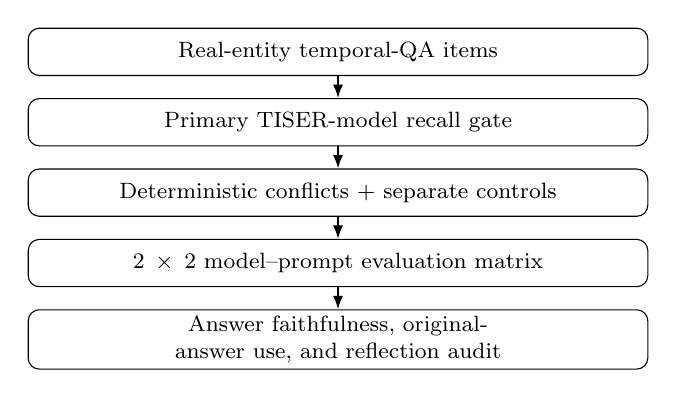
\begin{tikzpicture}[
  node distance=2.8mm,
  box/.style={draw, rounded corners, align=center, font=\footnotesize, text width=77mm, inner sep=2.4pt, minimum height=6mm},
  arr/.style={-{Latex[length=1.7mm]}, semithick}
]
\node[box] (n1) {Real-entity temporal-QA items};
\node[box, below=of n1] (n2) {Primary TISER-model recall gate};
\node[box, below=of n2] (n3) {Deterministic conflicts $+$ separate controls};
\node[box, below=of n3] (n4) {$2\times2$ model--prompt evaluation matrix};
\node[box, below=of n4] (n5) {Answer faithfulness, original-answer use, and reflection audit};
\draw[arr] (n1)--(n2);
\draw[arr] (n2)--(n3);
\draw[arr] (n3)--(n4);
\draw[arr] (n4)--(n5);
\end{tikzpicture}
\caption{Context--Memory Conflict is an inference-only evaluation pipeline. Controls preserve the answer and are kept separate from genuine conflicts.}
\label{fig:pipeline}
\end{figure}

\subsection{Extension 2: Tennis-Domain Adaptation}

\paragraph{Dataset creation and processing.}
The tennis collection is synthetic and was created with ChatGPT using the \href{https://developers.openai.com/api/docs/models/gpt-5.5}{GPT-5.5 model} in two stages using the prompts in Appendix~\ref{app:tennis-prompts}. First, the model generated raw context--question--answer triples from scratch using the raw-example prompt. Second, it received training examples together with their gold answers and generated supervised TISER reasoning, timeline, reflection, and answer traces using the trace-generation prompt. The examples were generated synthetically rather than drawn from an external tennis corpus. The dataset is released under \href{https://creativecommons.org/licenses/by/4.0/}{CC BY 4.0}; repository code is released under MIT.

The generated records are checked, categorised, deduplicated, and divided into disjoint training, model-selection, and final-holdout splits while keeping exact duplicate groups together. Reasoning traces are generated only for training examples. Separate semantic and trace audits assess whether the source questions are answerable and whether the generated supervision supports the supplied answers. Section~\ref{sec:experimental-setup} gives the exact split, recovery, conversion, and audit procedures.

\paragraph{Adaptation strategies.}
We first compare standard prompting, TISER prompting, and tennis-only adaptation at the smaller model scale. At the larger scale, we test direct transfer of the original TISER adapter and continued adaptation on tennis traces. We then evaluate whether the selected tennis-adapted model retains its original-domain capability; replay training is conditional on evidence of forgetting.

\section{Experimental Setup}
\label{sec:experimental-setup}

\subsection{Data and Evaluation}

After a 2,048-token filter, TISER training uses 54,488 examples. The test set has 19,214 in-domain examples and 2,800 ToT-semantic OOD examples. The conflict subset is constructed from 15,898 real-entity in-domain items and is evaluated on the 1,056 conflicts and 120 controls described above.

\subsection{Tennis Data, Trace, and Parsing Details}

The processing pipeline audits the schema, assigns identifiers and rule-based categories, converts records to standard and TISER-compatible prompts, checks duplicates, and performs a category- and exact-duplicate-group-aware 70/10/20 split with seed~42. The three disjoint files contain 785 training examples, 113 examples in \texttt{tennis\_dev.json}, and 224 examples in \texttt{tennis\_test.json}, jointly covering all 1,122 records. In the reported experiments, the 224-record test file is the model-selection split, while the 113-record development file is reserved as the final holdout. Trace generation is restricted to the training split.

The 785-record training split is the candidate pool for supervised trace creation; it is not itself the file used for optimization. It partitions exactly as $50+600+135=785$. Train positions 0--49 have valid traces from an initial pilot and support only pilot/smoke runs. Train positions 50--649 are the disjoint 600-record trace collection used by both reported tennis adaptations. For positions 650--784, requests were prepared in batches 13--15 but no generated outputs are present, so those 135 examples could not be used as supervised trace targets. The repository therefore contains traces for 650 unique training records overall, but the reported models use only the 600-record full-run file.

Of the 600 traces used for training, 200 lacked the requested tags and were wrapped around their generated reasoning and supplied gold answer; 26 records were recovered from 19 malformed JSONL lines. These repairs restore file structure rather than validate temporal correctness, which is assessed separately by the trace audit. The conversion CLI's \texttt{reported} mode reproduces the processed files, including their legacy answer-format instruction. At inference time, the evaluator replaces that instruction in memory with a strict-XML contract requiring the final answer inside \texttt{<answer>} tags; the stored files are not modified. The strict-XML conversion mode writes this explicit instruction into newly processed files and is reserved for new experiments.

The evaluator first applies TISER's \texttt{<answer>} parser. If no usable tagged answer is found, it attempts fallback extraction from common instruct-style answer phrases, the last standalone yes/no response for yes/no categories, and concise event spans for designated span-answer categories. A successfully recovered fallback is treated as usable rather than malformed. Tennis-specific normalization then handles rankings, minute durations, punctuation, and articles before EM and F1 are computed.

The 113 examples in \texttt{tennis\_dev.json} have no training traces, were never used for gradient updates, and were excluded from model selection for use as the final holdout. The repository contains no evidence of earlier model-performance use of this split, but its complete historical independence cannot be externally verified. The 224 examples in \texttt{tennis\_test.json} likewise have no training traces and never affect gradients, but they were used to evaluate every completed condition and rank the 7B candidates; they therefore serve as the selection split. All selection evaluations use the same 224 IDs in the same order. The complete 785-record split and unused generation requests document the deterministic 1,122-record partition, pilot provenance, and trace coverage.

\subsection{Tennis Semantic and Trace Audits}

Structural validity does not establish that a gold answer is uniquely entailed by its context or that a generated trace supports its answer. We therefore completed two UI-mediated, blinded file-batch audits. The semantic audit covers 1,121 unique context--question--gold payloads, mapping to all 1,122 source rows because two rows are identical. The trace audit covers all 650 available training traces: the 50-record pilot and the separate 600-record collection used for the reported adaptations. Semantic labels are \emph{supported}, \emph{wrong gold}, \emph{underdetermined}, \emph{inconsistent}, and \emph{unscorable}; trace labels are \emph{supported}, \emph{unsupported reasoning}, \emph{contradictory}, and \emph{unscorable}.

For each audit, Judge A and Judge B ran in separate tasks in the Codex app~\cite{openai2026codexapp}. The UI displayed \texttt{gpt-5.6-sol} with high reasoning effort for each task. Each task received only its assigned bundle, pass-specific rubric, and the common task prompt reproduced in Appendix~\ref{app:model-judge-audits}. Every scorable decision required item-specific reasoning and an exact quotation from the relevant source field. Hashes associate each response with its batch, item, source, and prompt. The two passes disagreed on 9 semantic items and 12 traces. A third task adjudicated every disagreement; the semantic workflow also adjudicated every proposed gold-answer change, producing 12 semantic and 12 trace adjudications in total. All expected decisions passed schema, identity, and exact-evidence validation.

These audits assess the data used to train the reported adapters; they do not alter the training inputs. Semantic adjudication produces alternative scoring views while preserving the original source files. The Codex UI did not expose a verifiable backend snapshot or decoding settings, so these details are unavailable. All primary and adjudication decisions used the same displayed model label, and no human calibration was performed. Agreement across the two passes therefore measures repeatability within one model family rather than independent or human-validated correctness; exact quotations validate evidence provenance, not the labels themselves.

\subsection{Models, Training, and Decoding}

Table~\ref{tab:settings} consolidates the training hyperparameters. Models generate the reasoning, timeline, reflection, and answer tags autoregressively in one pass. Prompt tokens are excluded from the training loss so that supervision targets only the structured completion. LoRA~\cite{hu2022lora} targets the $q$, $k$, $v$, and $o$ attention projections. The reproduction uses no base-model quantization; the 7B continued-adaptation run loads the base in 4-bit precision. All reported answer generations are greedy. Reproduction and conflict runs allow up to 768 new tokens; tennis evaluation allows up to 768 tokens at 0.5B and 256 at 7B.

\begin{table}[t]
\centering
\caption{Hyperparameters for the reported trained adapters. Micro.$\times$GA gives the per-device microbatch and gradient-accumulation factor.}
\label{tab:settings}
\setlength{\tabcolsep}{2.3pt}
{\footnotesize
\begin{tabular}{lrrrrl}
\toprule
\textbf{Run} & \textbf{$n$} & \textbf{Ep.} & \textbf{Updates} & \textbf{Micro.$\times$GA} & \textbf{Quant.} \\
\midrule
TISER 7B & 54{,}488 & 3 & 10{,}215 & $8{\times}2$ & none \\
Tennis 0.5B & 600 & 1 & 600 & $1{\times}1$ & none \\
Continued 7B & 600 & 2 & 74 & $4{\times}4$ & 4-bit NF4 \\
\bottomrule
\end{tabular}

\vspace{0.4em}
\begin{tabular}{@{}lp{0.72\columnwidth}@{}}
\textbf{Optimisation} & Paged 8-bit AdamW; learning rate $2{\times}10^{-4}$; cosine schedule; warmup ratio 0.03; weight decay 0; sequence limit 2,048; seed 42. \\
\textbf{LoRA} & Rank 16; $\alpha=32$; dropout 0.05; targets $q$, $k$, $v$, and $o$ projections; no bias. \\
\textbf{Checkpointing} & Enabled for TISER 7B and continued 7B; disabled for tennis 0.5B. The 4-bit run uses double quantisation. \\
\end{tabular}
}
\end{table}

The continued-adaptation condition was selected from 22 unique candidates evaluated on the same 224-record selection split. The main 18-candidate grid crossed one to three epochs, learning rates $\{5{\times}10^{-5},1{\times}10^{-4},2{\times}10^{-4}\}$, and gradient accumulation $\{4,8\}$ with per-device batch size~4 and LoRA dropout 0.05. Four additional one-epoch candidates used dropout 0.0 with learning rates $\{1{\times}10^{-4},2{\times}10^{-4}\}$ and gradient accumulation $\{4,8\}$. This common selection split enables direct comparison. Continued adaptation achieved the highest selection-set score and led two runners-up by one correct answer. Its fixed-protocol rerun reaches 0.728 EM and 0.852 F1 on this split. The selected adapter was then kept unchanged and evaluated once on the separate 113-record final holdout.

The retention experiment defines up to five conditions. C0 is the original TISER adapter, and C1 is the selected tennis-adapted model. If the retention gate detects forgetting, C1R is a fresh current-environment reproduction trained on the same 600 tennis traces; R25 is the replay condition trained on those traces plus 200 original-TISER examples; and R25-T is a replay sensitivity condition matched as closely as possible to C1R's supervised-token exposure.

The protocol first compares C0 and C1 on a predefined seed-42 sample of up to 100 items per original-TISER split. A 10,000-resample paired interval for the five-split macro-EM difference triggers C1R and R25 training only when its upper bound is below $-0.02$; a lower bound above $-0.02$ stops as non-inferior, and other intervals stop as inconclusive. If triggered, C1R and R25 both start from C0 and run for 74 updates under the same current environment. R25-T is run only when R25 supervised-token exposure differs from C1R by more than 10\%. The completed semantic audit retains the original 113-record final-holdout view from \texttt{tennis\_dev.json} and the 224-record selection view from \texttt{tennis\_test.json}, without proposed changes or exclusions. The final campaign evaluates the applicable fixed conditions on the 113 tennis inputs; original-domain retention is reported from the predefined sample. The reflection and trace audits are independent of this evaluation. Its results are not used for further model selection or training.

\subsection{Conflict Sampling and Reflection Audit}

Closed-book recall uses five samples with temperature~0.7 and top-$p$~0.9. The TISER-trained model's majority answer is retained when it occurs at least three times and matches the original gold answer, yielding 571 eligible source items. Deterministic edits produce 1,056 genuine conflicts---203 date-range shifts, 520 entity substitutions, and 333 interval reversals---plus 120 answer-preserving controls. The subsequent $2\times2$ model--prompt matrix uses one greedy decode per constructed row. Context-faithful EM/F1 measures agreement with the edited answer; original-answer EM measures agreement with the pre-edit answer and primary TISER-model memory. Malformed rate records non-compliance with the expected output format. Malformed does not necessarily mean unusable: if the parser recovers an answer span, that span remains in the accuracy calculation.

We use constructed-row bootstrap confidence intervals with 2,000 resamples and seed~42, plus row-paired McNemar tests for the two headline axes. The 1,176 rows originate from 546 source items, and the bootstrap resamples rows independently rather than clustering multiple variants from one source. The resulting intervals and tests describe the constructed rows and may understate source-level uncertainty; they are not treated as independent-question population inference.

The earlier Claude-based aggregate is excluded from the present results because its exact model version, complete prompt, and row-level decisions are unavailable. We instead conducted a UI-mediated audit of the saved outputs. The audit deduplicates the two 1,176-row TISER-prompt cells into 2,295 non-empty reflections, which map back to 2,348 source rows; four malformed source rows are retained as unscorable. Judge A and Judge B ran in separate Codex tasks configured in the UI as \texttt{gpt-5.6-sol} with high reasoning effort. Each task received only its blinded reflection bundle and a conservative pass-specific rubric, without model condition, conflict class, answer correctness, performance, or the other pass's decisions. Responses required an item-specific rationale and an exact source substring for every positive label. Hashes associate the evidence with its batch, item, source, response, and prompt; the shared judge prompt is reproduced once in Appendix~\ref{app:model-judge-audits}.

The primary decision is one of three labels: \emph{explicit conflict}, \emph{no explicit conflict}, or \emph{unscorable}. A positive label requires the reflection itself to acknowledge tension between supplied context and prior knowledge, memory, expectation, or an alternative factual answer; routine timeline checking is negative. The two passes disagreed on 66 of 2,295 reflections. A third Codex task, also configured as GPT-5.6 Sol with high reasoning, adjudicated those items from the source reflection and both primary decisions under the same conservative rule. All 66 adjudications passed the predefined schema and exact-evidence checks.

\subsection{Compute and Software}

The reproduction was trained on one H200 SXM GPU in bf16 for approximately 6.5 hours. Test and conflict generation used vLLM~\cite{kwon2023vllm} on an H100 SXM GPU; the full 22,014-example evaluation took approximately 17 minutes. Reported versions were PyTorch~2.4.1/CUDA~12.4, Transformers~4.46.3, PEFT~0.13.2, and TRL~0.12.2 for reproduction, and vLLM~0.22.0 with PyTorch~2.11/CUDA~13.0 for accelerated inference.

\section{Results}

\subsection{Baseline Reproduction}

Table~\ref{tab:baseline} reports the full in-domain evaluation of the reproduced TISER-trained condition. Our macro-EM is 0.033 below the paper, while macro-F1 is 0.005 higher; this implementation-level reproduction is therefore in a similar aggregate performance regime, but it does not reproduce every original baseline or ablation and its error profile differs substantially on TGQA.

\begin{table}[t]
\centering
\caption{TISER reproduction on five in-domain splits. \emph{Paper} is the comparable Qwen2.5-7B+TISER result; ToT-semantic (OOD EM 0.381) is excluded from the macro.}
\label{tab:baseline}
\setlength{\tabcolsep}{3.7pt}
{\footnotesize
\begin{tabular}{lrcccc}
\toprule
& & \multicolumn{2}{c}{\textbf{Ours}} & \multicolumn{2}{c}{\textbf{Paper}} \\
\cmidrule(lr){3-4}\cmidrule(lr){5-6}
\textbf{Split} & \textbf{$n$} & \textbf{EM} & \textbf{F1} & \textbf{EM} & \textbf{F1} \\
\midrule
TGQA            & 3{,}316 & 0.571 & 0.870 & 0.845 & 0.942 \\
TempReason L2   & 5{,}397 & 0.907 & 0.929 & 0.855 & 0.875 \\
TempReason L3   & 4{,}426 & 0.961 & 0.974 & 0.915 & 0.949 \\
TimeQA easy     & 2{,}997 & 0.980 & 0.989 & 0.979 & 0.983 \\
TimeQA hard     & 3{,}078 & 0.970 & 0.981 & 0.961 & 0.972 \\
\midrule
\rowcolor{gray!18}
\textbf{Macro (5)} & 19{,}214 & \textbf{0.878} & \textbf{0.949} & 0.911 & 0.944 \\
\bottomrule
\end{tabular}
}
\end{table}

TGQA combines low EM (0.571) with much higher F1 (0.870). Partially correct or differently formatted answers are compatible with this pattern, but the substantial 0.274 EM gap from the paper remains unexplained. The repository does not preserve the row-level annotations needed to substantiate a previously reported adjusted-accuracy estimate, so we omit that estimate rather than treating it as a reproducible result.

\subsection{Context--Memory Conflict}

Table~\ref{tab:conflict} makes the 1,056 genuine conflicts the primary population and reports the 120 controls separately. On this common TISER-selected population, the TISER-trained model with the TISER prompt reaches faithful-EM 0.774, compared with 0.348 for the vanilla model under a standard prompt. Relative to the same-model standard prompt, TISER prompting is associated with +0.214 EM; relative to vanilla weights under the same TISER prompt, TISER-trained weights are associated with +0.249. The latter is not a fully controlled model effect because eligibility is defined by the TISER-trained model's recall.

\begin{table}[t]
\centering
\caption{Run matrix on the TISER-selected population. Conflict metrics use only genuine conflicts ($n=1{,}056$); control EM is separate ($n=120$). Orig.-EM scores the pre-edit answer, equal to the primary TISER-model memory. $\Delta$EM is relative to base+standard.}
\label{tab:conflict}
\setlength{\tabcolsep}{1.4pt}
{\footnotesize
\begin{tabular}{lccccc}
\toprule
\textbf{Condition} & \textbf{Faith-EM} & \textbf{Faith-F1} & \textbf{Orig.-EM} & \textbf{$\Delta$EM} & \textbf{Ctrl.\ EM} \\
\midrule
Base + standard & 0.348 & 0.579 & 0.295 & --     & 0.658 \\
Base + TISER    & 0.525 & 0.718 & 0.228 & +0.176 & 0.883 \\
TISER + standard & 0.560 & 0.759 & 0.251 & +0.211 & 0.700 \\
\rowcolor{gray!18}
\textbf{TISER + TISER} & \textbf{0.774} & \textbf{0.914} & \textbf{0.153} & \textbf{+0.425} & \textbf{0.900} \\
\bottomrule
\end{tabular}
}
\end{table}

For continuity with the original aggregation, faithful-EM over conflicts \emph{plus} controls is 0.380, 0.561, 0.574, and 0.787 in table order. The previously reported rise from 0.380 to 0.787 therefore includes controls; the conflict-only comparison is 0.348 to 0.774. On all 1,176 constructed rows, the prompt-axis difference is +0.213 and the model-axis difference is +0.225. Row-paired McNemar tests give $p<10^{-40}$ for both contrasts, but repeated variants from the same source make these values unsuitable as source-level evidence; the large descriptive effect sizes are the primary result.

Figures~\ref{fig:conflict-matrix} and~\ref{fig:conflict-classes} separate the model--prompt comparison from the conflict-type analysis.

\begin{figure}[t]
\centering
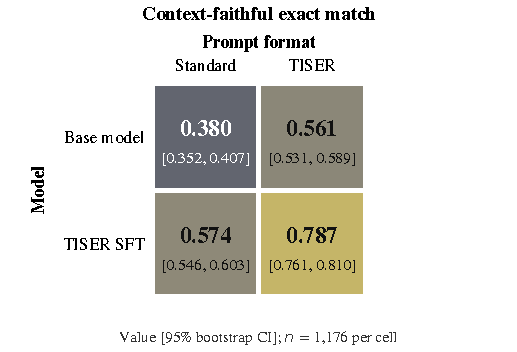
\includegraphics[width=\columnwidth]{figures/conflict_run_matrix.pdf}
\caption{Context-faithful exact match across the $2{\times}2$ model--prompt matrix on the TISER-selected population. Each cell reports EM and a constructed-row bootstrap 95\% interval over 1,176 rows, including 120 controls. Variants from one source are not clustered, so the intervals may understate source-level uncertainty.}
\label{fig:conflict-matrix}
\end{figure}

\subsection{Conflict Type and Reflection}

Table~\ref{tab:perclass} isolates the three genuine conflict types for the strongest condition. On this constructed benchmark, date shifts and entity swaps are largely solved, whereas order reversal is a clear weakness and the only class for which memorised EM exceeds faithful EM. The contrast does not by itself identify the mechanism: the transformations differ, and broad question-type pooling can make some entity substitutions semantically conspicuous.

\begin{figure}[t]
\centering
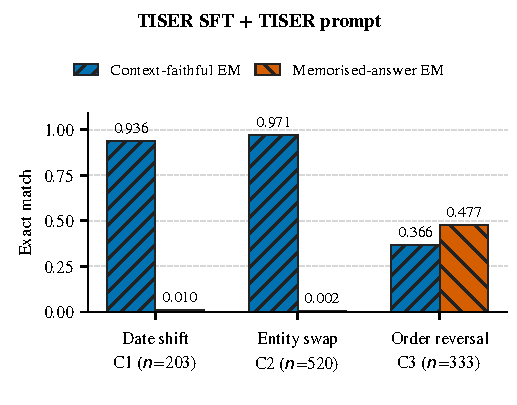
\includegraphics[width=\columnwidth]{figures/conflict_per_class.pdf}
\caption{Faithful and memorised-answer exact match for the TISER-fine-tuned model with the TISER prompt on the three genuine conflict classes (controls excluded). Order reversals are the only class in which memorised-answer EM exceeds context-faithful EM; this is a benchmark-specific empirical contrast rather than a causal diagnosis.}
\label{fig:conflict-classes}
\end{figure}

\begin{table}[t]
\centering
\caption{Genuine-conflict results for TISER model+prompt. \emph{Refl.} is the secondary LLM-judge conflict-naming rate.}
\label{tab:perclass}
\setlength{\tabcolsep}{5.0pt}
{\footnotesize
\begin{tabular}{lrccc}
\toprule
\textbf{Class} & \textbf{$n$} & \textbf{Faith-EM} & \textbf{Mem-EM} & \textbf{Refl.} \\
\midrule
C1 date shift      & 203 & 0.936 & 0.010 & 0.020 \\
C2 entity swap     & 520 & 0.971 & 0.002 & 0.006 \\
\rowcolor{gray!18}
C3 order reversal  & 333 & 0.366 & 0.477 & 0.087 \\
\midrule
\textbf{All conflicts} & 1{,}056 & \textbf{0.774} & \textbf{0.153} & \textbf{0.034} \\
\bottomrule
\end{tabular}
}
\end{table}

\begin{table}[t]
\centering
\caption{Completed GPT-5.6 Sol reflection audit. Conflict and control columns report explicit flags; disagreement compares the two primary passes; silent counts faithful genuine-conflict answers without a flag. Denominators exclude three unscorable genuine-conflict reflections for Base+TISER and one unscorable control for TISER+TISER.}
\label{tab:reflection-audit}
\setlength{\tabcolsep}{2.4pt}
{\footnotesize
\begin{tabular}{lrrrr}
\toprule
\textbf{Condition} & \textbf{Conflict} & \textbf{Control} & \textbf{Disagree} & \textbf{Silent} \\
\midrule
Base + TISER & 87/1{,}053 & 3/120 & 41/1{,}173 & 543/554 \\
\rowcolor{gray!18}
TISER + TISER & 36/1{,}056 & 3/119 & 25/1{,}175 & 810/817 \\
\bottomrule
\end{tabular}
}
\end{table}

Under the model-judge criterion, the replacement audit finds explicit conflict acknowledgement in 87/1,053 scorable genuine conflicts for the vanilla model with the TISER prompt (8.26\%, Wilson 95\% CI 6.75--10.08\%) and 36/1,056 for the TISER-trained model with the TISER prompt (3.41\%, 2.47--4.68\%). Control false-positive rates are 3/120 (2.50\%, 0.85--7.09\%) and 3/119 (2.52\%, 0.86--7.15\%), respectively. In the strongest answer-faithfulness condition, conflict flags remain concentrated in C3: 4/203 C1 items (1.97\%), 3/520 C2 items (0.58\%), and 29/333 C3 items (8.71\%). Among its 817 faithful genuine-conflict answers, 810 have no explicit flag, yielding a 99.14\% silent-override rate (98.24--99.58\%). The corresponding operational rate for the vanilla model with the TISER prompt is 543/554, or 98.01\% (96.48--98.89\%); because selection did not require stable vanilla-model recall, not every such row demonstrates override of that model's own memory. The 3.41\% genuine-conflict rate is descriptively close to the 2.52\% control rate, so these results support rarity and C3 concentration but do not establish reliable discrimination between genuine conflicts and controls. The separate control arm reaches faithful-EM 0.900 in the strongest condition; because its answer equals the primary memory by construction, it measures preservation of answerability rather than conflict resolution. A silent override remains a behavioural description, not proof of an internal conflict-resolution mechanism.

\subsection{Tennis-Domain Adaptation}

Table~\ref{tab:tennis} reports all completed 224-example selection-set runs. At 0.5B, prompting alone does not help, while tennis-only training gives a modest gain. At 7B, the original TISER adapter provides the direct-use reference and the fixed-protocol rerun of continued adaptation adds 0.147 EM and 0.151 F1. All 22 candidates were evaluated on the same 224-record selection split, enabling direct comparison, and continued adaptation achieved the highest selection-set score. Because no unadapted Qwen2.5-7B condition was evaluated, the absolute performance of the original TISER adapter cannot be attributed specifically to TISER training.

\begin{table}[t]
\centering
\caption{Tennis temporal QA on the 224-record selection split stored in \texttt{tennis\_test.json}. Deltas are against the first row within each model-size block; \emph{Malformed} is an output count.}
\label{tab:tennis}
\setlength{\tabcolsep}{3.4pt}
{\footnotesize
\begin{tabular}{lccccc}
\toprule
\textbf{Condition} & \textbf{EM} & \textbf{F1} & \textbf{$\Delta$EM} & \textbf{$\Delta$F1} & \textbf{Malf.} \\
\midrule
\multicolumn{6}{l}{\emph{Qwen2.5-0.5B-Instruct}} \\
Base, standard prompt   & 0.379 & 0.472 & -- & -- & 0 \\
Base, TISER prompt      & 0.375 & 0.420 & $-$0.004 & $-$0.052 & 5 \\
\rowcolor{gray!10}
Tennis-only adapter     & 0.464 & 0.516 & +0.085 & +0.045 & 0 \\
\midrule
\multicolumn{6}{l}{\emph{Qwen2.5-7B-Instruct}} \\
Original TISER & 0.580 & 0.701 & -- & -- & 0 \\
\rowcolor{gray!18}
\textbf{Continued adaptation} & \textbf{0.728} & \textbf{0.852} & \textbf{+0.147} & \textbf{+0.151} & 0 \\
\bottomrule
\end{tabular}
}
\end{table}

\subsection{Retention and Final Holdout}

The retention evaluation sampled 100 records from each of six original-TISER splits. The primary comparison uses the five in-domain splits ($n=500$); ToT-semantic remains separate OOD evidence. C0 reaches 0.880 macro-EM and C1 reaches 0.876, a difference of $-0.004$ with a paired 95\% interval of $[-0.028,0.020]$. This interval satisfies neither the clear-forgetting nor the non-inferiority rule, so the gate is inconclusive and C1R, R25, and R25-T are not trained. On the separate 100-record ToT-semantic sample, EM changes from 0.410 to 0.320 and F1 from 0.410 to 0.347; this split does not enter the gate.

The final tennis evaluation uses all 113 model-judge-supported holdout records. Continued adaptation raises EM from 0.575 to 0.735 and F1 from 0.677 to 0.834. The paired EM difference is 0.159 (95\% CI 0.080--0.239), and the exact McNemar test gives $p=0.000277$. Table~\ref{tab:retention-final} reports the paired summaries. Exploratory category results show that EM rises from 0.467 to 0.800 on duration questions ($n=15$), 0.250 to 0.400 on immediate before/after questions ($n=20$), 0.391 to 0.609 on first/last questions ($n=23$), and 0.821 to 0.923 on yes/no ordering questions ($n=39$), while overlap EM remains 0.909 ($n=11$). These small category samples identify where the aggregate gain occurs but are not separately powered confirmatory tests.

\begin{table}[t]
\centering
\caption{Original-domain retention and final tennis-holdout results. Differences are C1$-$C0; intervals use 10,000 paired bootstrap resamples with seed~42.}
\label{tab:retention-final}
\setlength{\tabcolsep}{2.8pt}
{\footnotesize
\begin{tabular}{lrrrr}
\toprule
\textbf{Evaluation} & \textbf{C0} & \textbf{C1} & \textbf{$\Delta$} & \textbf{95\% CI} \\
\midrule
Retention macro EM & 0.880 & 0.876 & $-$0.004 & [$-$0.028, 0.020] \\
Retention macro F1 & 0.946 & 0.936 & $-$0.010 & [$-$0.028, 0.007] \\
\rowcolor{gray!18}
Tennis holdout EM & 0.575 & 0.735 & +0.159 & [0.080, 0.239] \\
\rowcolor{gray!18}
Tennis holdout F1 & 0.677 & 0.834 & +0.157 & [0.082, 0.232] \\
\bottomrule
\end{tabular}
}
\end{table}

\subsection{Tennis Audit Results}

Table~\ref{tab:tennis-audits} summarizes the completed two-pass audits. The semantic decisions map back to all 1,122 source rows: all 113 final-holdout records in \texttt{tennis\_dev.json} and all 224 selection records in \texttt{tennis\_test.json} are model-judge supported, so both evaluation views retain their original labels and denominators. All 18 semantic concerns occur in training: 13 records are underdetermined, four have a model-adjudicated proposed gold-answer change, and one is internally inconsistent. Fourteen of these records belong to the reported 600-record training set and four to the untraced tail; none belongs to the 50-record pilot. The four proposed changes are \texttt{tennis\_000704}, \texttt{tennis\_000716}, and \texttt{tennis\_000885} from ``Yes'' to ``No,'' and \texttt{tennis\_000948} from ``Djokovic hit two aces'' to ``Sinner elected to receive.'' These proposed changes were not substituted into the training files used for the reported runs.

\begin{table}[t]
\centering
\caption{Completed tennis model-judge audits. Label abbreviations are U: underdetermined; WG: wrong gold; I: inconsistent; UR: unsupported reasoning; C: contradictory.}
\label{tab:tennis-audits}
\setlength{\tabcolsep}{2.8pt}
{\footnotesize
\begin{tabular}{lrrlr}
\toprule
\textbf{Audit} & \textbf{$n$} & \textbf{Supported} & \textbf{Other final labels} & \textbf{A/B dis.} \\
\midrule
Semantic (unique) & 1{,}121 & 1{,}103 & 13 U; 4 WG; 1 I & 9 \\
Trace & 650 & 632 & 14 UR; 4 C & 12 \\
\bottomrule
\end{tabular}
}
\end{table}

The trace audit supports all 50 pilot traces. Within the 600 traces used for the reported adaptations, 582 are supported, 14 contain unsupported reasoning, and four are contradictory. Combining the semantic and trace decisions, 21 distinct records in the 600-record training set have at least one concern; 579 are supported by both model audits. A cross-audit comparison also finds six records for which the semantic and trace decisions imply different readings: three have a supported semantic record but an unsupported trace, while three have a flagged semantic record but a supported trace. This audit examines the training data used by the reported models rather than measuring the causal effect of individual records: that effect cannot be inferred without retraining or ablation, and the model-judge decisions are not human certification.

\section{Discussion and Limitations}

The reproduction recovers a similar aggregate in-domain regime but not an identical error profile: in particular, the large TGQA EM gap remains unexplained and no claim is made that every original baseline or ablation was reproduced. More importantly, the two extensions answer different questions. The conflict probe provides strong descriptive evidence that prompt and weight conditions change use of supplied context on the constructed benchmark without making reflection an explicit contradiction detector. The tennis study establishes a continued-adaptation gain over the original TISER adapter; it does not establish that the original adapter outperforms an unadapted 7B model.

Threats to internal validity arise from benchmark construction and statistical dependence. Conflict eligibility is based on the TISER-trained model, so the vanilla-model rows are evaluated on a TISER-selected population and do not always represent conflict with the vanilla model's own stable memory. The entity-swap pool enforces broad question-type matching but not fine-grained semantic type, potentially making some C2 edits unusually conspicuous. Multiple variants originate from one source item, while the reported bootstrap and McNemar analyses operate on constructed rows; their uncertainty may therefore be anti-conservative at the source level. The large point-estimate differences remain descriptive results, but model-axis and conflict-type contrasts should not be read as fully isolated causal effects.

Threats to measurement validity include EM's sensitivity to answer form and the use of one model family for both primary audit passes and adjudication. Exact quotations and hashes make the model-judge decisions traceable, but neither those checks nor inter-pass agreement establish human-calibrated accuracy. The exact judge backend snapshot and decoding settings are unavailable. Greedy decoding also provides one subject-model output per condition.

External validity is limited by the confident-recall filter, the synthetic tennis distribution, and evaluation of one model family at two sizes. The tennis study uses different starting conditions at 0.5B and 7B, so it is not a controlled test of scale; the missing unadapted 7B baseline also prevents attribution of direct-use tennis performance specifically to prior TISER training. The audits identify concerns in 21 records inside the 600-record training set, whose size reflects an operational cutoff rather than a principled sample size; their causal effect remains unmeasured. The best 7B setting was selected on 224 records and evaluated once on a separately reserved 113-record holdout, although complete historical non-use of that holdout cannot be externally verified. The retention interval establishes neither clear forgetting nor non-inferiority, so the conditional replay branch was not executed and no claim is made about replay effectiveness. Training variability remains unmeasured because each adapter represents one training run.

\section{Conclusion}

We implemented the TISER pipeline and recovered a similar aggregate in-domain performance regime, while observing a substantial unresolved TGQA EM discrepancy. On a common population selected through the TISER-trained model's recall, structured prompting and TISER-trained weights were associated with greater use of edited context. Model-judged reflections rarely acknowledged the conflict explicitly, and order reversal remained a clear weakness on the constructed benchmark. On the separately reserved 113-record tennis holdout, continued adaptation improved EM from 0.575 to 0.735 over direct use of the original TISER adapter. This comparison establishes the adaptation gain but, without an unadapted 7B baseline, does not isolate the contribution of prior TISER training. Original-domain retention was inconclusive, so the conditional replay branch was not executed. Overall, contextual answer use, explicit conflict acknowledgement, and domain-specific adaptation are distinct capabilities and should be evaluated separately.

\newpage
\section{Reproducibility}

The repository provides command-line workflows for data preparation, training, evaluation, scoring, auditing, and statistical analysis. It records canonical configurations, seed~42, resolved settings, predictions, metrics, and available environment metadata for the reported models and results. Dataset provenance, licences, generation prompts, and trace coverage are documented separately.

The audit records retain the shared task prompt, pass-specific rubrics, original responses, hashes, decisions, adjudications, row-level outputs, and summaries. The reflection, semantic, and trace audits contain 4,590/66, 2,242/12, and 1,300/12 primary judgments/adjudications, respectively; the semantic audit also provides the 113- and 224-record evaluation views.

The Colab notebook implements the conditional retention and final-evaluation workflow with resumable stages. The completed branch evaluates C0 and C1 on the predefined retention sample, records the inconclusive gate without starting replay training, and evaluates both fixed adapters on the 113-record tennis holdout. File hashes associate each run with its data, configuration, adapter, and scoring view.

\clearpage
\onecolumn
\appendices

\section{Tennis Data-Generation Prompts}
\label{app:tennis-prompts}

The exact, verbatim prompts are versioned in the repository as
\href{https://github.com/thestbobo/tiser_temporal_reasoning_extension/blob/main/docs/extensions/tennis_domain_adaptation/RAW_GENERATION_PROMPT.md}{\texttt{RAW\_GENERATION\_PROMPT.md}} and
\href{https://github.com/thestbobo/tiser_temporal_reasoning_extension/blob/main/docs/extensions/tennis_domain_adaptation/TRACE_GENERATION_PROMPT.md}{\texttt{TRACE\_GENERATION\_PROMPT.md}}.
The compact excerpts below preserve the task, output contract, and principal constraints; the linked files are authoritative for exact reproduction.

\subsection{Stage 1: Raw Example Creation}

\begin{lstlisting}[style=prompt]
ABBREVIATED PROTOCOL (not the verbatim prompt)

Task: Generate batches of exactly 50 synthetic professional-tennis
temporal-QA examples.

Output: one valid JSON array with records
{"context":"...", "question":"...", "answer":"..."}

Requirements:
- Each self-contained context has 3--6 sentences and at least
  three temporally related events.
- The answer must be short, unique, and inferable only from context.
- Cover before/after, first/last, duration, overlap, and tournament
  progression questions, with varied difficulty and answer polarity.
- Avoid ambiguity, external knowledge, and near duplicates.
- Do not output reasoning, timelines, reflections, Markdown, or text
  outside the JSON array.
\end{lstlisting}

ChatGPT-5.5 used the full linked prompt to generate the 1,122 raw records before schema auditing, categorisation, and splitting. The omitted prompt text enumerates tennis scenarios, target category proportions, examples, and a pre-output quality checklist.

\subsection{Stage 2: TISER Trace Generation}

\begin{lstlisting}[style=prompt]
ABBREVIATED PROTOCOL (not the verbatim prompt)

Input: question_id, category, context, question, and gold_answer.
Output: one JSONL record per example:
{"question_id":"...", "output":"..."}

Required output structure:
<reasoning>...
<timeline>...</timeline>
<reflection>...</reflection>
...</reasoning>
<answer>GOLD_ANSWER</answer>

Use only the supplied context; reason about the required temporal
relations; construct a chronological timeline; verify the gold answer
in the reflection; invent no event, date, entity, or relation; preserve
question_id; and return JSONL only.
\end{lstlisting}

The full linked prompt generated the supervised traces. The final 600 records exactly match batches 1--12 in order. Nineteen malformed physical JSONL lines covering 26 records were repaired, and 200 outputs that lacked the requested XML-like tags were mechanically wrapped using their existing text and supplied gold answer. All 600 final rows pass structural and gold-answer-equality checks; those checks do not establish semantic entailment.
\section{Model-Judge Prompt and Adjudication}
\label{app:model-judge-audits}

The reflection, semantic, and trace audits used one shared task prompt, pasted unchanged into the separate Judge A, Judge B, and adjudicator tasks. Its exact text is versioned as
\href{https://github.com/thestbobo/tiser_temporal_reasoning_extension/blob/main/docs/GPT56_SOL_AUDIT_TASK_PROMPT.md}{\texttt{GPT56\_SOL\_AUDIT\_TASK\_PROMPT.md}}; each task additionally received only its assigned JSON bundle containing the audit-specific, pass-specific rubric and blinded items.

\begin{lstlisting}[style=prompt]
ABBREVIATED PROTOCOL (not the verbatim prompt)

Use only the assigned bundle. Do not inspect the repository, another
judge pass, previous decisions, or experiment outputs. Judge every item
individually under its batch rubric without keyword or default-label
heuristics.

For every item, return its unchanged audit_id and source_sha256, one
allowed label, an item-specific rationale, and any required exact source
quotation. Provide a corrected answer only for semantic wrong_gold.
For reflection labels, distinguish explicit conflict from routine
timeline checking and record the permitted mention kind.

Validate every response file against its batch identity, schema, item
coverage, allowed labels, and exact-evidence requirements.
\end{lstlisting}

The excerpt states the audit contract; the linked file preserves the exact response schema, allowed mention kinds, interruption behaviour, and operator instructions used in all passes.
\subsection{Adjudication}

Judge A and Judge B were compared by item identity. Follow-up bundles contained
the original source and both decisions for every disagreement, plus every proposed
\emph{wrong gold} decision in the semantic audit. A third independent task,
configured in the UI as \texttt{gpt-5.6-sol} with high reasoning effort,
reapplied the relevant rubric without majority voting. The workflow adjudicated
66 reflection, 12 semantic, and 12 trace decisions. All 90 passed the label,
identity, hash, and exact-quotation checks.

\begin{thebibliography}{00}

\bibitem{bazaga2025tiser}
A. Bazaga, R. Blloshmi, B. Byrne, and A. de Gispert,
"Learning to Reason Over Time: Timeline Self-Reflection for Improved Temporal Reasoning in Language Models,"
in \emph{Proceedings of the 63rd Annual Meeting of the Association for Computational Linguistics (Volume 1: Long Papers)}, Vienna, Austria, 2025, pp. 28014--28033, doi: 10.18653/v1/2025.acl-long.1358. [Online]. Available: \url{https://aclanthology.org/2025.acl-long.1358/}

\bibitem{xiong2024tgqa}
S. Xiong, A. Payani, R. Kompella, and F. Fekri,
"Large Language Models Can Learn Temporal Reasoning,"
in \emph{Proceedings of the 62nd Annual Meeting of the Association for Computational Linguistics (Volume 1: Long Papers)}, Bangkok, Thailand, 2024, pp. 10452--10470, doi: 10.18653/v1/2024.acl-long.563. [Online]. Available: \url{https://aclanthology.org/2024.acl-long.563/}

\bibitem{tan2023tempreason}
Q. Tan, H. T. Ng, and L. Bing,
"Towards Benchmarking and Improving the Temporal Reasoning Capability of Large Language Models,"
in \emph{Proceedings of the 61st Annual Meeting of the Association for Computational Linguistics (Volume 1: Long Papers)}, Toronto, Canada, 2023, pp. 14820--14835, doi: 10.18653/v1/2023.acl-long.828. [Online]. Available: \url{https://aclanthology.org/2023.acl-long.828/}

\bibitem{chen2021timeqa}
W. Chen, X. Wang, and W. Y. Wang,
"A Dataset for Answering Time-Sensitive Questions,"
in \emph{Proceedings of the Neural Information Processing Systems Track on Datasets and Benchmarks}, vol. 1, Round 2, 2021. [Online]. Available: \url{https://datasets-benchmarks-proceedings.neurips.cc/paper/2021/hash/1f0e3dad99908345f7439f8ffabdffc4-Abstract-round2.html}

\bibitem{hu2022lora}
E. J. Hu, Y. Shen, P. Wallis, Z. Allen-Zhu, Y. Li, S. Wang, L. Wang, and W. Chen,
"LoRA: Low-Rank Adaptation of Large Language Models,"
in \emph{International Conference on Learning Representations}, 2022. [Online]. Available: \url{https://openreview.net/forum?id=nZeVKeeFYf9}

\bibitem{qwen2024qwen25}
A. Yang et al.,
"Qwen2.5 Technical Report,"
\emph{arXiv preprint arXiv:2412.15115}, 2024, doi: 10.48550/arXiv.2412.15115. [Online]. Available: \url{https://arxiv.org/abs/2412.15115}

\bibitem{kwon2023vllm}
W. Kwon, Z. Li, S. Zhuang, Y. Sheng, L. Zheng, C. H. Yu, J. E. Gonzalez, H. Zhang, and I. Stoica,
"Efficient Memory Management for Large Language Model Serving with PagedAttention,"
in \emph{Proceedings of the ACM SIGOPS 29th Symposium on Operating Systems Principles}, Koblenz, Germany, 2023, pp. 611--626, doi: 10.1145/3600006.3613165. [Online]. Available: \url{https://doi.org/10.1145/3600006.3613165}

\bibitem{openai2026codexapp}
OpenAI,
"Introducing the Codex app," Feb. 2, 2026. [Online]. Available:
\url{https://openai.com/index/introducing-the-codex-app/}.

\end{thebibliography}

\end{document}
